\section{Fundamental concepts in geometry}

$\cdot$ This is the 2nd reading seminar of the series, held by Prof. Pigati on April 1st $\cdot $\\

What follows is a set of informal definitions of objects like manifolds, charts and tangent space that are at the basis of the geometric framework introduced above. 

Given $n \in \mathbb{N}$, a n-dimensional \textit{manifold} $\mathcal{M}^n$ is, roughly, something that looks like the Euclidean space $\mathbb{R}^n$ at small scale. When defining manifolds, we don't actually use a notion of distance (metric), instead we use topological notions and define a ``small scale" in terms of open sets. 

\begin{definition}[Manifold] \label{def:mnf}%or structure of manifold? 
    Given a topological space $M^n$ (Hausdorff*, second countable), a structure of an n-dimensional manifold is given by:
    \begin{itemize}
        \item[i.] a collection $\{U_i\}_{i \in I}$ of open sets $U_i \subseteq M$ such that $M= \bigcup_{i \in I} U_i$;
        \item[ii.] for each $i$, a bijective map $\varphi_i : U_i \longrightarrow V_i \subseteq \mathbb{R}^n$;
        \item[iii.] $\varphi_i \circ \varphi^{-1}_j : \varphi_j (U_i \cap U_j) \longrightarrow \varphi_i(U_i \cap U_j)$ is $C^\infty$ \,\,\,\, \textit{(compatibility property)}
    \end{itemize}
    Where you can think of the property of being ``Hausdorff" as the points in the space being distinguishable; and the compatibility property ensures we can define what is a smooth function on our manifold. \\

\end{definition}

\begin{example}
    Take $U\subset \mathbb{R}^n$ open. $\mathcal{M}^n := U$ is a n-dimensional manifold with open cover $\{U\}$ and chart $\{id: U\longrightarrow U\}$.
\end{example}

\begin{example}\label{ex:sn_1}
    Take the unitary n-dimensional sphere $S^n = \{x \in \mathbb{R}^{n+1}:|x| = 1\}$. Given $p \in S^n$, we define the emisphere related to $p$ by cutting the sphere in half with the hyperplane generated by the vector $p$ (the hyperplane orthogonal to it) where the origin $0$ lies, i.e. $U_p := \{x \in S^n : (x,p)>0\}$. Then, $\varphi_p:U_p \longrightarrow B_1(0)$ is a projection that ``flattens" the emisphere onto the hyperplane. 
\end{example}

\begin{example}[Guess the manifold]\label{ex:cyl}
    Take $M^2= U_1 \cup U_2$.\\
    $\varphi_1: U_1 \longrightarrow \mathbb{R} \times (0, 2\pi)$\\
    $\varphi_2: U_2 \longrightarrow \mathbb{R} \times (0, 2\pi)$\\
    $\varphi_1(U_1 \cap U_2) = \mathbb{R}\times (\pi, 2\pi)$\\
    $\varphi_2  \circ \varphi_1^{-1}(x,y) := (x, y-\pi)$\\
    
    \textbf{Solution:} We can deduce that our manifold $M$ is a cylinder. The charts $\varphi_1$ and $\varphi_2$ will be maps from the manifold to the cylinder minus one line (to ensure bijection). %si?
\end{example}

\begin{example}[Guess the manifold]\label{ex:sn_2}
    Take $M^2= U_1 \cup U_2$.\\
    $\varphi_1: U_1 \longrightarrow \mathbb{R}^2 $\\
    $\varphi_2: U_2 \longrightarrow \mathbb{R}^2$\\
    $\varphi_1(U_1 \cap U_2) = \varphi_2(U_1 \cap U_2) = \mathbb{R}^2 \setminus \{0\}$\\
    $\varphi_2  \circ \varphi_1^{-1}(x) = \frac{x}{|x|^2}$\\
    
    \textbf{Solution:} We can deduce that our manifold is the 2-dimensional sphere $S^2$, where $\varphi_1 $is given by the sphere without the point at the north pole, and $\varphi_2$ is given by removing the south pole. The two maps project the manifold onto the plane cutting it in half (the plane where the equator lies). 
\end{example}

\begin{definition}[Charts]
    The maps $\varphi_i:U_i \longrightarrow V_i$ used in definition \ref{def:mnf} are called charts. The inverse maps $\varphi_i^{-1}$ are called parametrizations. 
\end{definition}

    The main conceptual idea is that for any point $x \in M^n$ in the manifold, you can find an open set $U_i$ that is omeomorphic to an open subset of the Euclidean space $\mathbb{R}^n$. Figure \ref{fig:mnf} helps visualizing this idea. 
    Then, we can think of charts as maps allowing us to find (multiple sets of) ``coordinates" for points on the manifold. Indeed, the inverse of a chart is a parametrization in the sense that it maps some parameters - vectors in $\mathbb{R}^n$ - to points in our manifold. What we hope is that the combination of charts defined on the same region on the manifold is smooth (compatibility property), in order to define a \textit{smooth} manifold (we could hope for any other property like continuity or $C^7$, and to enforce it we would impose it on charts in the same way). 


\begin{definition}[Atlas and maximal atlas]
A collection of charts is called an \textit{atlas}. Any atlas can be uniquely extended to a maximal atlas, which is one that is not contained in any other atlas.
\end{definition}

\begin{remark}
    Recall the examples above: the two structures we have defined on the manifold $S^n$ are the same, i.e. they give the same maximal atlas. 
\end{remark}

\begin{example}
    Here's instead an example of incompatible charts. Take $M=\mathbb{R}$ and the charts $id:M\longrightarrow \mathbb{R}$ and $\psi: M\longrightarrow \mathbb{R} : \psi(x)=x^3$. Then we get $id \circ \psi^{-1}(x) = \sqrt[3]{x} \notin C^\infty.$
\end{example}

\begin{definition}[Smoothness]
    Let $M,N$ be two manifolds such that:
    \begin{itemize}
        \item[] $M$ has atlas $\{\varphi_i\}_{i\in  I}:U_i \longrightarrow \mathbb{R}^n$
        \item[] $N$ has atlas $\{\psi_j\}_{j\in  J}:V_j\longrightarrow \mathbb{R}^n$
    \end{itemize}
    Given $p\in M$, $f:M \longrightarrow N$ is smooth if $\exists U_i \ni p$ and $\exists W_j \ni f(p), W_j \subseteq \mathbb{R}^n,$ such that the map
    \[\psi_j \circ f \circ \varphi_i^{-1}: \varphi_i(f^{-1}(W_j)) \longrightarrow W_j\] %i'm not sure it should be W_j here but rather psi(Wj)
    is smooth.\\
    Moreover, using compatibility of charts we can replace ``$\exists$" with ``$\forall$".
\end{definition}

Now, we turn to defining  what a tangent space is. approximated to a tangent space. 


\begin{figure}
    \centering
    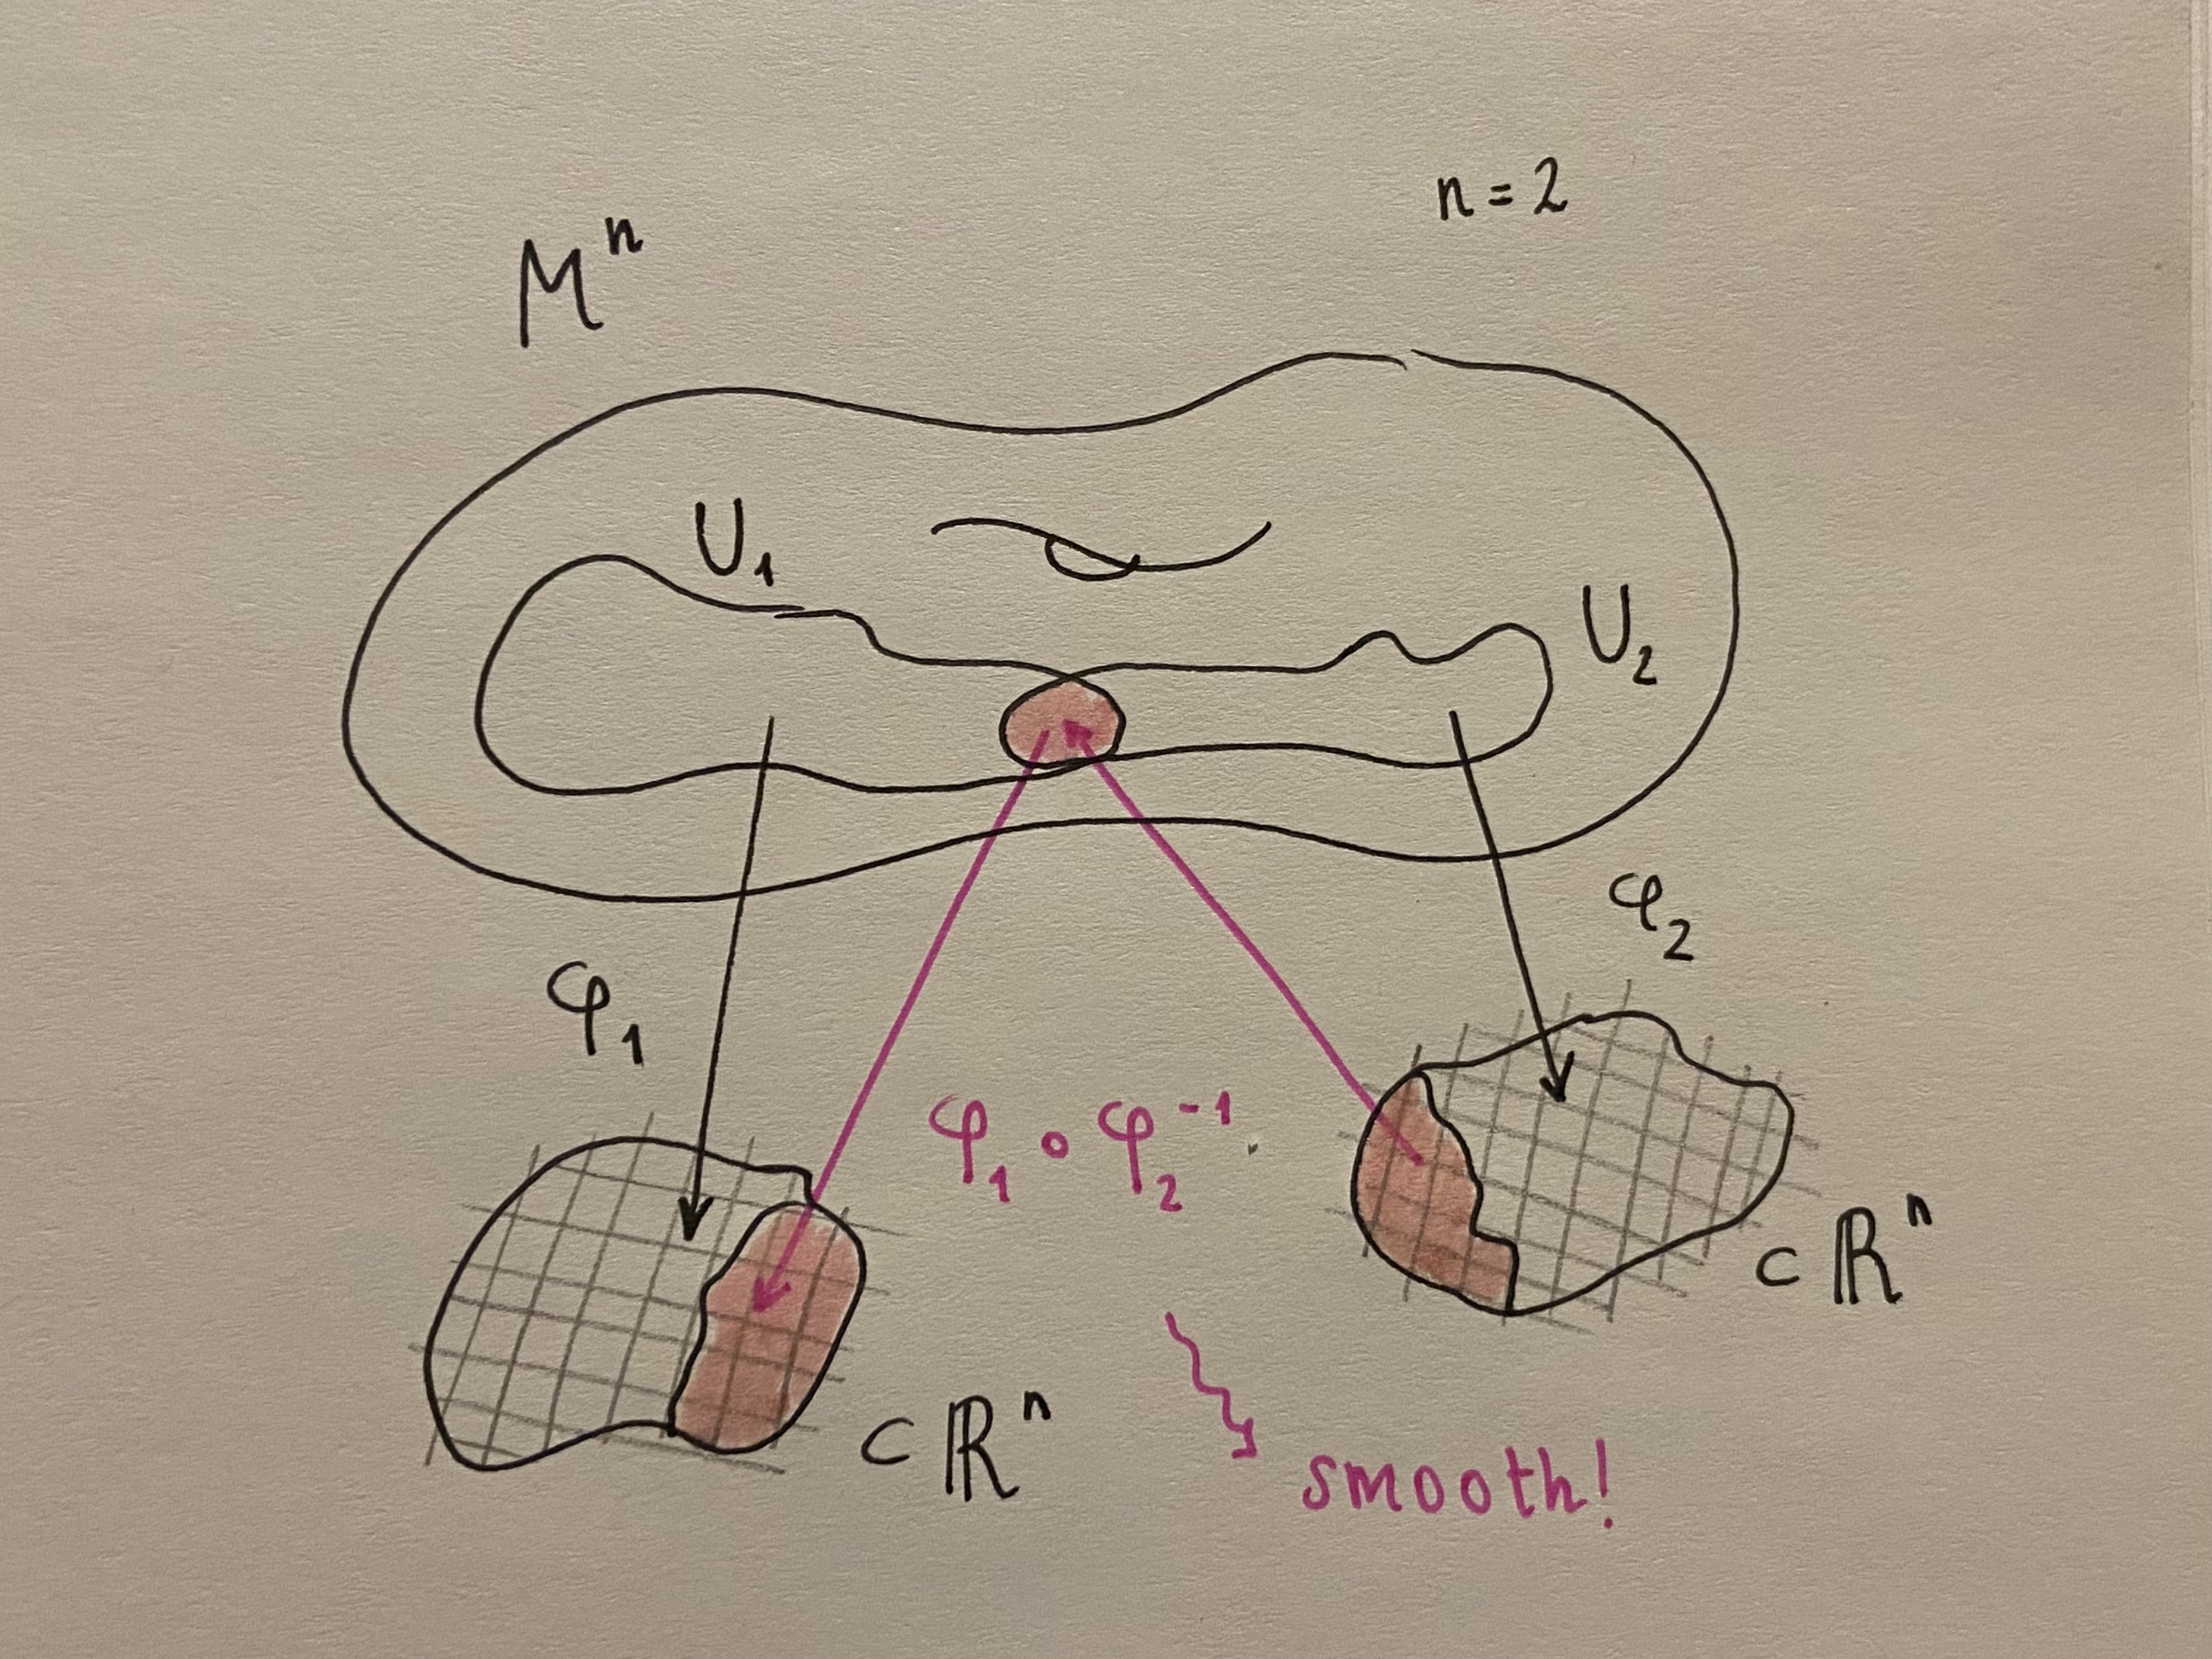
\includegraphics[width=0.5\linewidth]{images/manifold.png}
    \caption{Visual representation of a manifold. The two sets in the lower part are subsets of the Euclidean space, i.e. charts. What you would like is that the pink map ($\varphi_2  \circ \varphi_1^{-1}$) is smooth, so that the two coordinate system defined on the pink region of the manifold ($U_1 \cap U_2$) are compatible.}
    \label{fig:mnf}
\end{figure}